\subsection{2021年2月19日}
\paragraph{\href{https://www.51voa.com/VOA_Special_English/japan-starts-covid--vaccinations-86319.html}{原文}}

\begin{figure}[H]
\centering
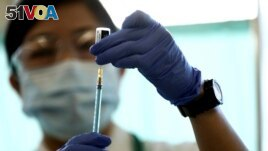
\includegraphics[scale=0.7]{004_voa_20210219.jpg}
\caption{A medical worker fills a syringe with a dose of the Pfizer-BioNTech COVID-19 vaccine at Tokyo Medical Center.(Behrouz Mehri/Pool Photo via AP)}
\end{figure}

By Dan Friedell
17 February 2021
Japan began giving COVID-19 vaccinations to its people on Wednesday. Many other developed countries began vaccination campaigns back in December.
Japan is behind other countries because it asked drug companies to carry out special clinical trials with Japanese people. The country only gave permission for the vaccine on Sunday.
The delay has some people worried that not enough Japanese people will be vaccinated before the proposed start of the delayed 2020 Tokyo Olympic Games.
The Games are now set to begin on July 23, after being delayed by one year because of the coronavirus health crisis.
The first people in Japan to get the vaccine -- made by Pfizer and BioNTech -- are medical workers, old people and people with health problems.
The rest of the Japanese public may be able to get a vaccine in the late spring or early summer.
Japan has a population of 127 million people. At the current rate, not enough people will have the vaccine by the start of the Olympics to make sure everyone is safe.
Officials are struggling to fight opposition among citizens to holding the Games. Recent public opinion studies in Japan found that about 80 percent of those questioned support canceling the Games completely or delaying them again.
But Japanese leaders, including Prime Minister Yoshihide Suga, say they want to move forward with the Games. They say the Olympics will be "proof of human victory against the pandemic."
Japan also wants to show the world it can hold the Olympics before China runs the 2022 Winter Olympics in Beijing. Those Games are set to start in less than one year.
Japan has dealt with the pandemic better than many Western countries. But a recent increase in cases has caused concern. Currently, some parts of Japan are under stronger restrictions than they faced during most of 2020.
Japan is still doing well compared to many other countries. About one person out of every 100,000 is testing positive for the virus. In the United States, that number is almost 25 out of 100,000.
One of the first Japanese people to get the vaccine was Dr. Kazuhiro Araki. He is the president of the Tokyo Medical Center.
He said it did not hurt, adding "I hope we feel more at ease."
Taro Kono is Japan's vaccine minister. He answered criticism about the slow start to the vaccination program by saying it was important to show the Japanese people it would be safe.
"So at the end of the day we might have started slower, but we think it will be more effective," he said.
Japanese leaders say they are working to develop more vaccines in Japan instead of using doses from other countries. More vaccine will arrive next week.
Almost 4 million health care workers are set to be vaccinated in March. Starting in April, the 36 million Japanese people aged 65 and older will be able to receive their shots.
I'm Dan Friedell.
Mari Yamaguchi wrote this story for The Associated Press. Dan Friedell adapted it for Learning English. Ashley Thompson was the editor.

\begin{messagebox}
Words in This Story
clinical trial - n. a test to determine the effectiveness of a new drug or medical technique
pandemic - n. an occurrence in which a disease spreads very quickly and affects a large number of people over a wide area or throughout the world
positive - adj. showing the presence of a particular germ, condition, or substance
dose - n. the amount of a medicine, drug, or vitamin that is taken at one time
\end{messagebox}

Japan began giving COVID-19 vaccinations to its people on Wednesday. Many other developed countries began vaccination campaigns back in December.
日本周三开始给本国民众接种新冠肺炎疫苗。许多发达国家去年12月就开始接种疫苗。
Japan is behind other countries because it asked drug companies to carry out special clinical trials with Japanese people. The country only gave permission for the vaccine on Sunday.
日本落后于其它国家,是因为它要求制药公司对日本人开展特殊的临床试验。该国在本周日才刚刚批准使用这种疫苗。
The delay has some people worried that not enough Japanese people will be vaccinated before the proposed start of the delayed 2020 Tokyo Olympic Games.
这种延误使一些人担心在被推迟的2020年东京奥运会拟开幕前,没有足够多的日本人能够接种疫苗。
The Games are now set to begin on July 23, after being delayed by one year because of the coronavirus health crisis.
这届奥运会由于新冠病毒危机被推迟一年之后,目前定于7月23日开幕。
The first people in Japan to get the vaccine -- made by Pfizer and BioNTech -- are medical workers, old people and people with health problems.
首批接种由辉瑞和BioNTech联合研制疫苗的日本民众包括医务人员、老年人以及存在健康问题的人士。
The rest of the Japanese public may be able to get a vaccine in the late spring or early summer.
其余日本民众也许能够在春末或夏初接种疫苗。
Japan has a population of 127 million people. At the current rate, not enough people will have the vaccine by the start of the Olympics to make sure everyone is safe.
日本有1.27亿人口。按目前的速度,到奥运会开幕时,没有足够多人士接种疫苗以确保每个人都安全。
Officials are struggling to fight opposition among citizens to holding the Games. Recent public opinion studies in Japan found that about 80 percent of those questioned support canceling the Games completely or delaying them again.
有关官员正在努力反驳市民对举办这届奥运会的反对意见。日本最近的民意调查发现,大约80%的被调查者支持完全取消或推迟奥运会。
But Japanese leaders, including Prime Minister Yoshihide Suga, say they want to move forward with the Games. They say the Olympics will be "proof of human victory against the pandemic."
但是包括首相菅义伟在内的日本领导人表示,他们希望继续推进这届奥运会。他们表示,这届奥运会将是“人类战胜大流行的证明。”
Japan also wants to show the world it can hold the Olympics before China runs the 2022 Winter Olympics in Beijing. Those Games are set to start in less than one year.
日本还想向世界展示,它有能力在中国举办2022年冬奥会之前举办本届奥运会。这两届奥运会将在不到1年时间内接连开幕。
Japan has dealt with the pandemic better than many Western countries. But a recent increase in cases has caused concern. Currently, some parts of Japan are under stronger restrictions than they faced during most of 2020.
日本在应对大流行方面要比许多西方国家都做得更好。但是最近的病例激增引发了人们的担忧。目前,日本某些地区受到了比2020年大部分时间都要更严格的限制。
Japan is still doing well compared to many other countries. About one person out of every 100,000 is testing positive for the virus. In the United States, that number is almost 25 out of 100,000.
与其它许多国家相比,日本表现仍然不错。每10万人中大约有1人对病毒呈阳性反应。在美国,这个数字是每10万人接近25人。
One of the first Japanese people to get the vaccine was Dr. Kazuhiro Araki. He is the president of the Tokyo Medical Center.
荒木和宏博士是首批接种该疫苗的日本人之一。他是东京医疗中心的总裁。
He said it did not hurt, adding "I hope we feel more at ease."
他说,接种疫苗不疼,并补充说,我希望大家更加安心。
Taro Kono is Japan's vaccine minister. He answered criticism about the slow start to the vaccination program by saying it was important to show the Japanese people it would be safe.
河野太郎是日本的疫苗大臣。他回应了人们对疫苗接种计划启动缓慢的批评。他说,向日本民众表明接种疫苗的安全,这一点很重要。
"So at the end of the day we might have started slower, but we think it will be more effective," he said.
他说:“所以到头来我们可能会启动缓慢,但是我们认为这样做会更有效。”
Japanese leaders say they are working to develop more vaccines in Japan instead of using doses from other countries. More vaccine will arrive next week.
日本领导人表示,他们正在努力开发更多日本疫苗,而不是使用其它国家的疫苗。下周会有更多疫苗面世。
Almost 4 million health care workers are set to be vaccinated in March. Starting in April, the 36 million Japanese people aged 65 and older will be able to receive their shots.
日本计划在3月份为400万医护人员接种疫苗。从4月开始,3600万名65岁及以上年龄的日本民众将能够接种疫苗。
